% !TEX root = ../main.tex

\section{Introducción}

% =========================================================
% 1. FUNDAMENTOS
% =========================================================
\subsection{Fundamentos y Métricas}

\begin{De}{Grafo ($G$)}{def:grafo}
Es una pareja de conjuntos $G=(V,A)$, donde:
\begin{itemize}
    \item $V$: Conjunto de \textbf{vértices} (o nodos).
    \item $A$: Conjunto de \textbf{aristas} (parejas de vértices).
\end{itemize}
\end{De}

\begin{De}{Grafo completo ($K_n$)}{def:completo}
Un grafo de $n$ vértices se llama \textbf{completo} (y se denota $K_n$) si cada pareja de vértices está conectada por una arista.
\end{De}

% !TEX root = ../main.tex

\begin{figure}[htbp]
  \centering
  \vspace*{-0.75\baselineskip}
  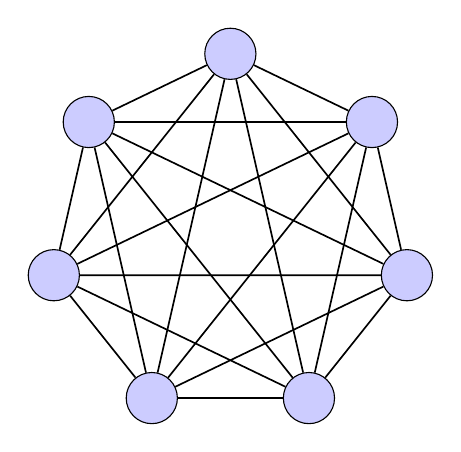
\begin{tikzpicture}[
    scale=1.0,
    every node/.style={transform shape},
    v/.style={circle, draw, fill=blue!20, minimum size=6.5mm, inner sep=0pt, font=\small},
    e/.style={draw, line width=0.6pt}
  ]
    % K7 (grafo completo con 7 vértices)
    \def\N{7}
    \def\R{2.3}

    % Vértices en un círculo
    \foreach \i in {1,...,\N} {
      \node[v] (v\i) at ({90 - 360*(\i-1)/\N}:\R) {};
    }

    % Aristas completas (i < j)
    \foreach \i in {1,...,\N} {
      \foreach \j in {\i,...,\N} {
        \ifnum\i<\j
          \draw[e] (v\i) -- (v\j);
        \fi
      }
    }
  \end{tikzpicture}
  \caption{Grafo completo $K_7$.}
  \label{fig:k7}
\end{figure}



\begin{Rmk}{Terminología de Aristas}{nota:aristas}
\begin{itemize}
    \item \textbf{Aristas paralelas:} Múltiples aristas que unen los mismos dos vértices.
    \item \textbf{Lazo (Loop):} Una arista que conecta un vértice consigo mismo.
\end{itemize}
\end{Rmk}

% !TEX root = ../main.tex

\begin{figure}[htbp]
  \centering
  \vspace{0.75\baselineskip}
  \vspace*{-0.75\baselineskip}
  \begin{tikzpicture}[
    scale=0.9,
    every node/.style={transform shape},
    v/.style={circle, draw, fill=blue!20, minimum size=7mm, inner sep=0pt, font=\small},
    lab/.style={font=\small\bfseries, fill=white, draw=none, inner sep=0pt},
    e/.style={draw, line width=0.45pt},
    w/.style={font=\scriptsize}
  ]

    % ---- SIMPLE
    \node[lab] (t1) at (0,2.25) {Simple};
    \node[v] (sa) at (0,1.35) {a};
    \node[v] (sb) at (1.5,1.10) {b};
    \node[v] (sc) at (-1.25,0.75) {c};
    \node[v] (sd) at (0,0.35) {d};
    \draw[e] (sa) -- (sb);
    \draw[e] (sa) -- (sd);
    \draw[e] (sc) -- (sd);

    % ---- MULTIGRAFO
    \begin{scope}[xshift=5.2cm]
      \node[lab] (t2) at (0,2.25) {Multigrafo};
      \node[v] (ma) at (0,1.35) {a};
      \node[v] (mb) at (1.5,1.10) {b};
      \node[v] (mc) at (-1.25,0.75) {c};
      \node[v] (md) at (0,0.35) {d};
      \draw[e] (ma) -- (mb);
      \draw[e] (ma) -- (md);
      \draw[e] (mc) -- (md);
      % aristas paralelas entre c y d
      \draw[e, bend left=25] (mc) to (md);
      \draw[e, bend right=25] (mc) to (md);
    \end{scope}

    % ---- PSEUDOGRAFO
    \begin{scope}[xshift=10.4cm]
      \node[lab] (t3) at (0,2.25) {Pseudografo};
      \node[v] (pa) at (0,1.35) {a};
      \node[v] (pb) at (1.5,1.10) {b};
      \node[v] (pc) at (-1.25,0.75) {c};
      \node[v] (pd) at (0,0.35) {d};
      \draw[e] (pa) -- (pb);
      \draw[e] (pa) -- (pd);
      \draw[e] (pc) -- (pd);
      % aristas paralelas y lazos
      \draw[e, bend left=25] (pc) to (pd);
      \draw[e, bend right=25] (pc) to (pd);
      \draw[e] (pb) to[out=20,in=-20,looseness=8] (pb);
      \draw[e] (pd) to[out=-120,in=-60,looseness=8] (pd);
    \end{scope}

    % ---- PONDERADO
    \begin{scope}[yshift=-3.6cm]
      \node[lab] (t4) at (0,2.25) {Ponderado};
      \node[v] (wa) at (0,1.35) {a};
      \node[v] (wb) at (1.5,1.10) {b};
      \node[v] (wc) at (-1.25,0.75) {c};
      \node[v] (wd) at (0,0.35) {d};
      \draw[e] (wa) -- node[w, above] {5} (wb);
      \draw[e] (wa) -- node[w, right] {10} (wd);
      \draw[e] (wc) -- node[w, left] {4} (wa);
      \draw[e] (wc) -- node[w, below left] {3} (wd);
    \end{scope}

    % ---- GRAFO DIRIGIDO
    \begin{scope}[xshift=5.2cm, yshift=-3.6cm]
      \node[lab] (t5) at (0,2.25) {Grafo dirigido};
      \node[v] (da) at (0,1.35) {a};
      \node[v] (db) at (1.5,1.10) {b};
      \node[v] (dc) at (-1.25,0.75) {c};
      \node[v] (dd) at (0,0.35) {d};
      \draw[e, -{Stealth[length=2.2mm]}] (da) -- (db);
      \draw[e, -{Stealth[length=2.2mm]}] (dc) -- (da);
      \draw[e, -{Stealth[length=2.2mm]}] (dd) -- (da);
      \draw[e, -{Stealth[length=2.2mm]}] (dc) -- (dd);
    \end{scope}

    % ---- MULTIGRAFO DIRIGIDO
    \begin{scope}[xshift=10.4cm, yshift=-3.6cm]
      \node[lab] (t6) at (0,2.25) {Multigrafo dirigido};
      \node[v] (mda) at (0,1.35) {a};
      \node[v] (mdb) at (1.5,1.10) {b};
      \node[v] (mdc) at (-1.25,0.75) {c};
      \node[v] (mdd) at (0,0.35) {d};
      \draw[e, -{Stealth[length=2.2mm]}] (mda) -- (mdb);
      \draw[e, -{Stealth[length=2.2mm]}] (mdc) -- (mda);
      \draw[e, -{Stealth[length=2.2mm]}] (mdc) -- (mdd);
      \draw[e, -{Stealth[length=2.2mm]}, bend left=20] (mda) to (mdd);
      \draw[e, -{Stealth[length=2.2mm]}, bend right=20] (mda) to (mdd);
    \end{scope}

  \end{tikzpicture}
  \caption{Tipos de grafos.}
  \label{fig:tipos-grafos}
\end{figure}


\subsubsection{Propiedades Métricas}

\begin{itemize}
    \item \textbf{Orden ($|V|$):} Número total de vértices.
    \item \textbf{Tamaño ($|A|$):} Número total de aristas.
    \item \textbf{Grado ($gr(v)$):} Número de aristas incidentes en un vértice $v$ (¡Ojo! los lazos suman 2 al grado).
\end{itemize}

\begin{De}{Isomorfismo}{def:isomorfismo-rep}
Dos representaciones se llaman \textbf{equivalentes} o \textbf{isomorfas} si corresponden al mismo conjunto de vértices y aristas.
\end{De}

Es decir, si existe una biyección entre sus vértices que preserva las aristas. 

\begin{Le}{del Apretón de Manos}{lema:apreton}
La suma de los grados de todos los vértices es igual al doble del número de aristas:
\[ \sum_{v \in V} gr(v) = 2|A| \]
\end{Le}

\begin{Co}{Paridad de los Grados}{cor:paridad}
El número de vértices de grado impar en cualquier grafo debe ser \textbf{par}. Si una secuencia de grados no cumple esto, el grafo no puede existir.
\end{Co}

% =========================================================
% 2. CONECTIVIDAD
% =========================================================
\subsection{Conectividad y Tipos Especiales}

\subsubsection{Caminos y recorridos}

\begin{De}{Camino}{def:camino}
Un \textbf{camino} es una sucesión de vértices $v_0,v_1,\dots,v_k$ tal que para todo $i=0,\dots,k-1$ existe una arista entre $v_i$ y $v_{i+1}$.
\end{De}

\begin{Rmk}{Camino simple}{nota:camino-simple}
Se dice que el camino es \textbf{simple} si no se repite ningún vértice.
\end{Rmk}
\begin{De}{Recorrido}{def:recorrido}
Un \textbf{recorrido} es un camino en el que no se repite ninguna arista.
\end{De}

\begin{De}{Circuito}{def:circuito}
Un \textbf{circuito} es un recorrido cerrado, es decir, un recorrido cuyo vértice inicial coincide con el final ($v_0=v_k$).
\end{De}

\begin{De}{Ciclo}{def:ciclo}
Un \textbf{ciclo} es un circuito en el que no se repite ningún vértice (salvo el primero/último).
\end{De}

\begin{De}{Grafo Conexo}{def:conexo}
Un grafo es conexo si existe un camino entre cualquier par de vértices del grafo.
\end{De}

\begin{Pro}{Condición de Suficiencia}{prop:suficiencia}
Para que un grafo de $N$ vértices sea conexo, el grado mínimo ($M$) de cada vértice debe cumplir:
\[ M \ge \frac{N-1}{2} \]
\end{Pro}

\subsubsection{Grafos Bipartitos}

\begin{De}{Grafo Bipartito}{def:bipartito}
El grafo cuyos vértices se pueden dividir en 2 subconjuntos de tal manera que entre los vértices del mismo conjunto no hay aristas.
\end{De}

\begin{figure}[H]
    \centering
    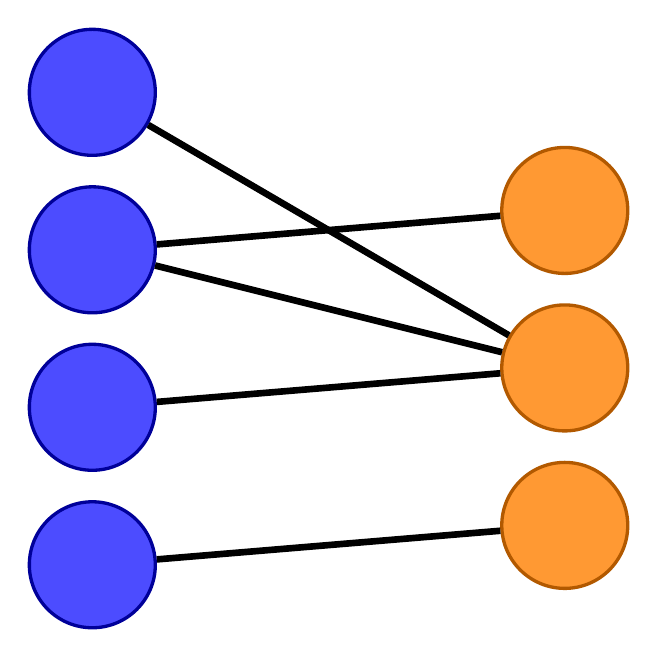
\begin{tikzpicture}[
        vertexA/.style={circle, draw=blue!60!black, fill=blue!70, very thick, minimum size=16mm},
        vertexB/.style={circle, draw=orange!70!black, fill=orange!80, very thick, minimum size=16mm},
        edge/.style={black, line width=2.4pt}
    ]
        % Conjunto A (izquierda)
        \node[vertexA] (a1) at (0,6) {};
        \node[vertexA] (a2) at (0,4) {};
        \node[vertexA] (a3) at (0,2) {};
        \node[vertexA] (a4) at (0,0) {};

        % Conjunto B (derecha)
        \node[vertexB] (b1) at (6,4.5) {};
        \node[vertexB] (b2) at (6,2.5) {};
        \node[vertexB] (b3) at (6,0.5) {};

        % Aristas (aprox. como en la imagen)

        \draw[edge] (a1) -- (b2);
        \draw[edge] (a2) -- (b1);
        \draw[edge] (a2) -- (b2);
        \draw[edge] (a3) -- (b2);
        \draw[edge] (a4) -- (b3);
    \end{tikzpicture}
    \caption{Ejemplo de grafo bipartito.}
    \label{fig:grafo-bipartito}
\end{figure}


\begin{De}{Grafo Bipartito Completo ($K_{n,m}$)}{def:bipartito-completo}
Un \textbf{grafo bipartito completo}, denotado $K_{n,m}$, es un grafo $G=(V,A)$ tal que existe una partición $V=V_1 \cup V_2$ con $V_1 \cap V_2 = \emptyset$, $|V_1|=n$ y $|V_2|=m$, y además:
\begin{itemize}
    \item No hay aristas entre vértices del mismo conjunto: si $v,v' \in V_1$ entonces $(v,v') \notin A$, y si $u,u' \in V_2$ entonces $(u,u') \notin A$.
    \item Todo vértice de $V_1$ está conectado con todo vértice de $V_2$: para todo $v \in V_1$ y $u \in V_2$, se tiene $(v,u) \in A$.
\end{itemize}
\end{De}

\begin{Rmk}{Número de Aristas}{nota:n-aristas}
En consecuencia, $K_{n,m}$ tiene exactamente $nm$ aristas.
\end{Rmk}

\subsubsection{Grafos Planos (Planares)}

\begin{De}{Grafos Planares}{def:planares}
El grafo se llama \textbf{planar} si se puede representar en el plano sin que las aristas se cruzen.
\end{De}

\begin{The}{Característica de Euler}{thm:euler}
Para cualquier grafo plano conexo se cumple siempre:
\[ V - A + C = 2 \]
Donde $V$: vértices, $A$: aristas, $C$: caras (regiones).
\end{The}

\begin{Pro}{Desigualdades de Planariedad}{prop:planariedad}
Si un grafo es plano simple y conexo con $V \ge 3$:
\begin{enumerate}
    \item $A \le 3V - 6$
    \item Si no tiene triángulos (ej. bipartitos): $A \le 2V - 4$
\end{enumerate}
\end{Pro}

\begin{The}{de Kuratowski}{thm:kuratowski}
Un grafo es plano si y solo si NO contiene subgrafos homeomorfos a $K_5$ o $K_{3,3}$.
\end{The}

% =========================================================
% 3. ÁRBOLES
% =========================================================
\subsection{Árboles}

\begin{De}{Árbol}{def:arbol}
\begin{itemize}
    \item Es un grafo conexo que no contiene ciclos.
    \item Es un grafo en el que para cada pareja de vértices existe un único recorrido que los une.
\end{itemize}
\end{De}

\begin{Pro}{Propiedades Fundamentales de los Árboles}{prop:arboles}
Sea $G$ un grafo con $n$ vértices. Las siguientes afirmaciones son equivalentes:
\begin{enumerate}
    \item $G$ es un árbol.
    \item Existe un \textbf{único camino simple} entre cada par de vértices.
    \item $G$ es conexo y cumple que $\mathbf{A = V - 1}$.
    \item $G$ no tiene ciclos y $A = V - 1$.
\end{enumerate}
\end{Pro}

\begin{The}{de Cayley}{thm:cayley}
Existen $n^{n-2}$ árboles etiquetados distintos de $n$ vértices.
\end{The}

\begin{De}{Secuencia de Prüfer}{prufer}

\end{De}


\subsection{Algoritmos y Matrices}

\begin{Pro}{Algoritmo de Havel-Hakimi}{prop:havel}
Determina si existe un grafo simple con una secuencia de grados dada.
\begin{enumerate}
    \item Ordenar grados de mayor a menor.
    \item Eliminar el primer grado $d$.
    \item Restar 1 a los siguientes $d$ grados de la lista.
    \item Repetir hasta obtener ceros (existe) o negativos (no existe).
\end{enumerate}
\end{Pro}

\subsubsection{Representación Matricial}

\begin{itemize}
    \item \textbf{Matriz de Adyacencia ($A$):} $A_{ij} = 1$ si hay arista.
    \begin{itemize}
        \item $(A^n)_{ij}$ indica el número de caminos de longitud $n$ entre $i$ y $j$.
    \end{itemize}
    \item \textbf{Matriz de Incidencia ($M$):} Vértices $\times$ Aristas.
\end{itemize}

\begin{Pro}{Relación Fundamental}{prop:matrices}
\[ M \cdot M^T = A + D \]
Donde $D$ es la matriz diagonal de grados.
\end{Pro}